\documentclass[oneside,a4paper,german,parskip=half]{scrbook}
\usepackage[latin1]{inputenc}

%Standartfont
\usepackage[T1]{fontenc}
\usepackage{libertine}

%Zusatzpaket f�r mathematische Ausdr�cke
\usepackage{amsmath}

%Zusatzfonts f�r mathbb usw.
\usepackage{amsfonts}
\usepackage{mathrsfs}

%Tikz/PGF Zeichnenpaket
\usepackage{pgf}
\usepackage{tikz}
\usetikzlibrary{mindmap,trees,decorations,decorations.pathreplacing,decorations.pathmorphing,calc,arrows,automata}

%F�r graphische Todos
\usepackage[colorinlistoftodos]{todonotes}
\newcommand{\Img}[1]{\todo[inline, nolist, color=black!40]{IMG: #1}}

\begin{document}
\tableofcontents
\newpage

\part{Informatik 2 - Sommersemester 2009}
\chapter{Grundlagen Informatik}
\section{29.04.2009}
\subsection{GI-29.04.2009-IMG-1}
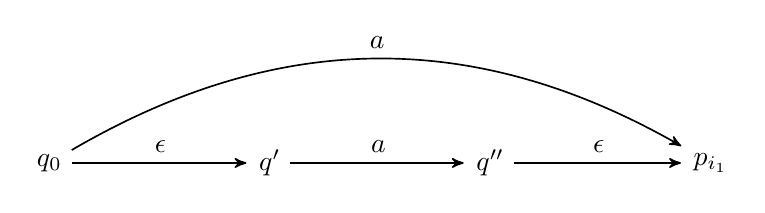
\begin{tikzpicture}[->,>=stealth',shorten >=1pt,auto,node distance=2.8cm,semithick]
\node (n0) {$q_0$};
\node (n1) [right of=n0] {$q'$};
\node (n2) [right of=n1] {$q''$};
\node (n3) [right of=n2] {$p_{i_1}$};

\path[->] (n0) edge node[above] {$\epsilon$} (n1);
\path[->] (n1) edge node[above] {$a$} (n2);
\path[->] (n2) edge node[above] {$\epsilon$} (n3);
\path[->] (n0) edge[bend left] node[above] {$a$} (n3);
\end{tikzpicture}
\Img{GI-29.04.2009-IMG-1}

\subsection{GI-29.04.2009-IMG-2}
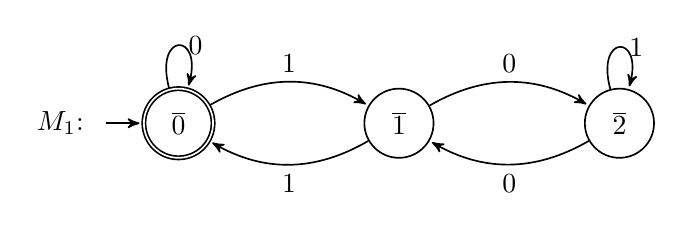
\begin{tikzpicture}[->,>=stealth',shorten >=1pt,auto,node distance=2.8cm,semithick]
\node[state, initial, initial text=, accepting] (n0) {$\overline{0}$};
\node[state] (n1) [right of=n0] {$\overline{1}$};
\node[state] (n2) [right of=n1] {$\overline{2}$};
\node [left of=n0, node distance=1.5cm] {$M_1$:};

\path[->] (n0) edge[loop above] node[right] {$0$} ();
\path[->] (n2) edge[loop above] node[right] {$1$} ();

\path[->] (n0) edge[bend left] node[above] {$1$} (n1);
\path[->] (n1) edge[bend left] node[below] {$1$} (n0);
\path[->] (n1) edge[bend left] node[above] {$0$} (n2);
\path[->] (n2) edge[bend left] node[below] {$0$} (n1);
\end{tikzpicture}
\Img{GI-29.04.2009-IMG-2.1}

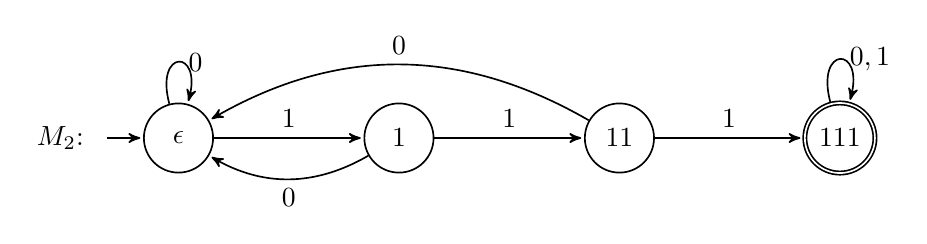
\begin{tikzpicture}[->,>=stealth',shorten >=1pt,auto,node distance=2.8cm,semithick]
\node[state, initial, initial text=] (n0) {$\epsilon$};
\node[state] (n1) [right of=n0] {$1$};
\node[state] (n2) [right of=n1] {$11$};
\node[state, accepting] (n3) [right of=n2] {$111$};
\node [left of=n0, node distance=1.5cm] {$M_2$:};

\path[->] (n0) edge[loop above] node[right] {$0$} ();
\path[->] (n3) edge[loop above] node[right] {$0,1$} ();

\path[->] (n0) edge node[above] {$1$} (n1);
\path[->] (n1) edge node[above] {$1$} (n2);
\path[->] (n2) edge node[above] {$1$} (n3);

\path[->] (n1) edge[bend left] node[below] {$0$} (n0);
\path[->] (n2) edge[bend right] node[above] {$0$} (n0);
\end{tikzpicture}
\Img{Gi-29.04.2009-IMG-2.2}

\subsection{GI-29.04.2009-IMG-3}
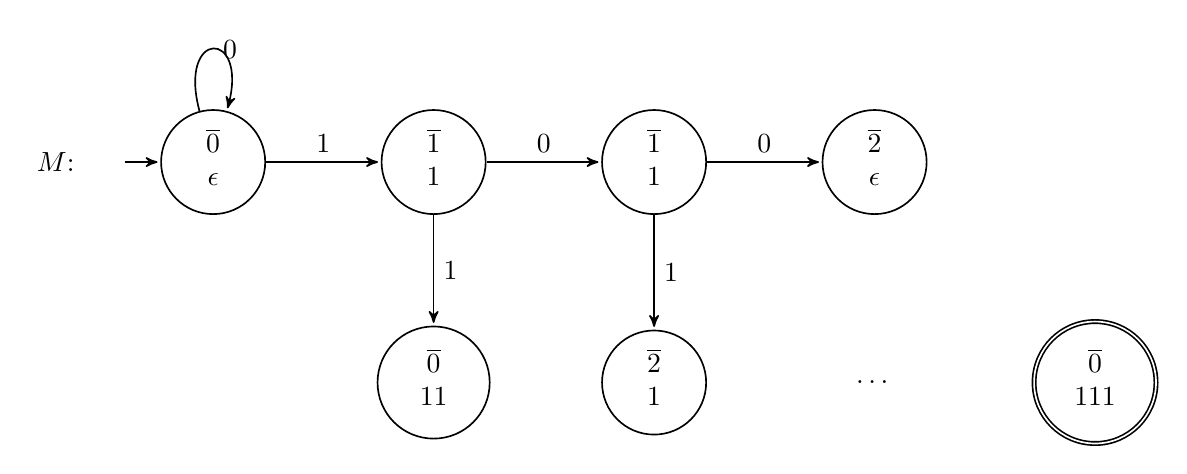
\begin{tikzpicture}[->,>=stealth',shorten >=1pt,auto,node distance=2.8cm,semithick]
\node[state, initial, initial text=] (n0) {$\begin{array}{c}\overline{0}\\\epsilon\end{array}$};
\node[state] (n1) [right of=n0] {$\begin{array}{c}\overline{1}\\1\end{array}$};
\node[state] (n2) [right of=n1] {$\begin{array}{c}\overline{1}\\1\end{array}$};
\node[state] (n3) [right of=n2] {$\begin{array}{c}\overline{2}\\\epsilon\end{array}$};
\node[state] (n4) [below of=n1] {$\begin{array}{c}\overline{0}\\11\end{array}$};
\node[state] (n5) [below of=n2] {$\begin{array}{c}\overline{2}\\1\end{array}$};
\node (n6) [right of=n5] {$\dots$};
\node[state, accepting] (n7) [right of=n6] {$\begin{array}{c}\overline{0}\\111\end{array}$};
\node[left of=n0,node distance=2.0cm] {$M$:};

\path[->] (n0) edge[loop above] node[right] {$0$} ();

\path[->] (n0) edge node[above] {$1$} (n1);
\path[->] (n1) edge node[above] {$0$} (n2);
\path[->] (n2) edge node[above] {$0$} (n3);
\path[->] (n1) edge node[right] {$1$} (n4);
\path[->] (n2) edge node[right] {$1$} (n5);
\end{tikzpicture}
\Img{GI-29.04.2009-IMG-3}

\section{30.04.2009}
\subsection{IMG-30.04.2009-IMG-1}
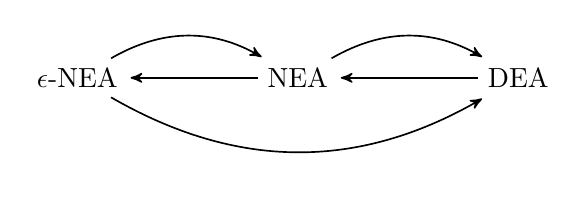
\begin{tikzpicture}[->,>=stealth',shorten >=1pt,auto,node distance=2.8cm,semithick]
\node (n0) {$\epsilon$-NEA};
\node (n1) [right of=n0] {NEA};
\node (n2) [right of=n1] {DEA};

\path[->] (n0) edge[bend left] (n1);
\path[->] (n1) edge[bend left] (n2);
\path[->] (n0) edge[bend right] (n2);
\path[->] (n1) edge (n0);
\path[->] (n2) edge (n1);
\end{tikzpicture}
\Img{GI-30.04.2009-IMG-1}

\subsection{IMG-30.04.2009-IMG-2}
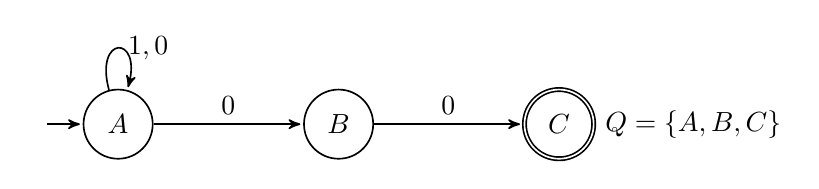
\begin{tikzpicture}[->,>=stealth',shorten >=1pt,auto,node distance=2.8cm,semithick]
\node[state, initial, initial text=] (n0) {$A$};
\node[state] (n1) [right of=n0] {$B$};
\node[state,accepting] (n2) [right of=n1] {$C$};
\node at (n2.east) [right,node distance=0.5cm] {$Q = \{A, B, C\}$};

\path[->] (n0) edge[loop above] node[right] {$1, 0$} ();
\path[->] (n0) edge node[above] {$0$} (n1);
\path[->] (n1) edge node[above] {$0$} (n2);
\end{tikzpicture}
\Img{GI-30.04.2009-IMG-2.1}

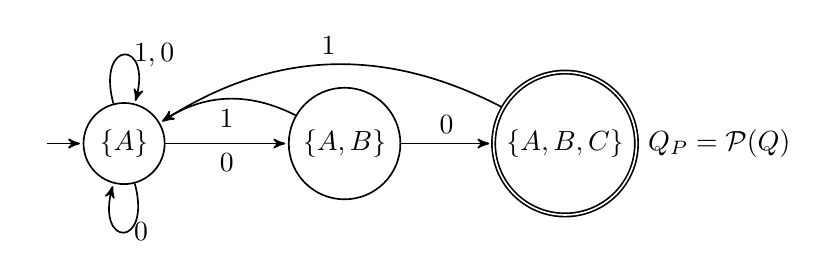
\begin{tikzpicture}[->,>=stealth',shorten >=1pt,auto,node distance=2.8cm,semithick]
\node[state, initial, initial text=] (n0) {$\{A\}$};
\node[state] (n1) [right of=n0] {$\{A, B\}$};
\node[state,accepting] (n2) [right of=n1] {$\{A, B, C\}$};
\node at (n2.east) [right,node distance=0.5cm] {$Q_P = \mathcal{P} (Q)$};

\path[->] (n0) edge[loop above] node[right] {$1, 0$} ();
\path[->] (n0) edge[loop below] node[right] {$0$} ();
\path[->] (n0) edge node[below] {$0$} (n1);
\path[->] (n1) edge node[above] {$0$} (n2);
\path[->] (n2) edge[bend right] node[above] {$1$} (n0);
\path[->] (n1) edge[bend right] node[below] {$1$} (n0);
\end{tikzpicture}
\Img{GI-30.04.2009-IMG-2.2}

\subsection{IMG-30.04.2009-IMG-3}
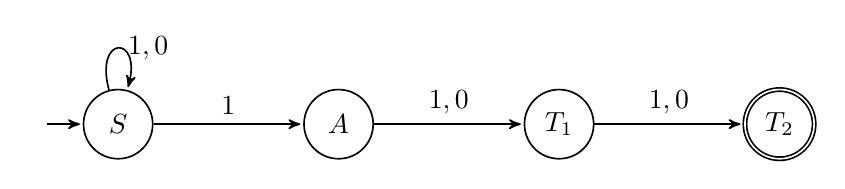
\begin{tikzpicture}[->,>=stealth',shorten >=1pt,auto,node distance=2.8cm,semithick]
\node[state, initial, initial text=] (n0) {$S$};
\node[state] (n1) [right of=n0] {$A$};
\node[state] (n2) [right of=n1] {$T_1$};
\node[state, accepting] (n3) [right of=n2] {$T_2$};

\path[->] (n0) edge[loop above] node[right] {$1,0$} ();
\path[->] (n0) edge node[above] {$1$} (n1);
\path[->] (n1) edge node[above] {$1,0$} (n2);
\path[->] (n2) edge node[above] {$1,0$} (n3);
\end{tikzpicture}
\Img{GI-30.04.2009-IMG-3.1}

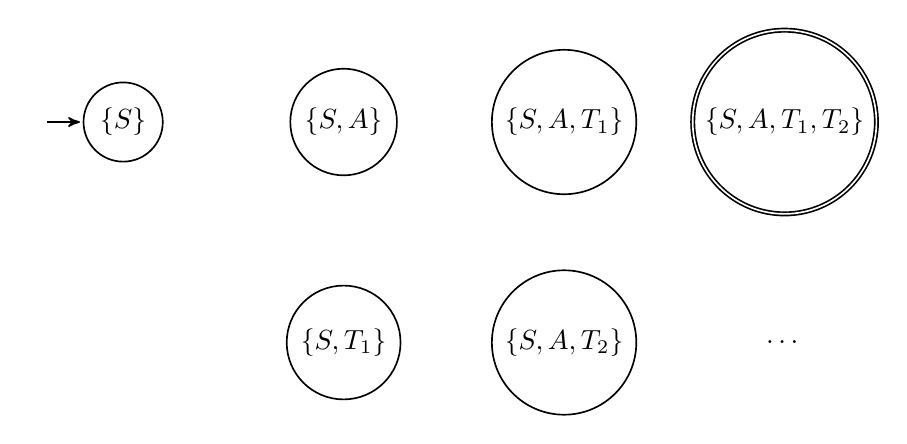
\begin{tikzpicture}[->,>=stealth',shorten >=1pt,auto,node distance=2.8cm,semithick]
\node[state,initial, initial text=] (n0) {$\{S\}$};
\node[state] (n1) [right of=n0] {$\{S, A\}$};
\node[state] (n2) [right of=n1] {$\{S, A, T_1\}$};
\node[state,accepting] (n3) [right of=n2] {$\{S, A, T_1, T_2\}$};
\node[state] (n4) [below of=n1] {$\{S, T_1\}$};
\node[state] (n5) [below of=n2] {$\{S, A, T_2\}$};
\node [right of=n5] {$\dots$};

\tikzloop{n0}{0}{above}{right}

\tikzedge{n0}{n1}{1}{}{above}
\tikzedge{n1}{n2}{1}{}{above}
\tikzedge{n2}{n3}{1}{}{above}
\tikzedge{n1}{n4}{0}{}{right}
\tikzedge{n4}{n5}{1}{}{above}
\end{tikzpicture}
\Img{GI-30.04.2009-IMG-3.2}

\section{05.05.2009}
\subsection{GI-05.05.2009-IMG-1}
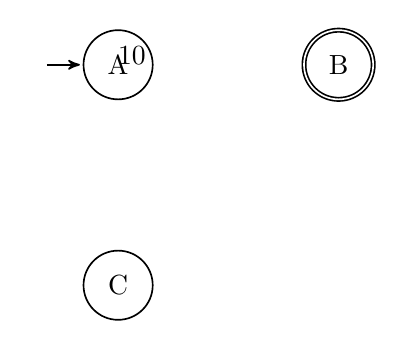
\begin{tikzpicture}[->,>=stealth',shorten >=1pt,auto,node distance=2.8cm,semithick]
\node[state,initial,initial text=] (A) {A};
\node[state, accepting] (B) [right of=A] {B};
\node[state] (C) [below of=A] {C};

\tikzloop{A}{$1$}{above}{};
\tikzloop{B}{$0$}{above}{};
\tikzedge{A}{B}{1}{}{};
\tikzedge{A}{C}{0}{}{};
\tikzedge{B}{C}{1}{}{};
\end{tikzpicture}
\Img{GI-05.05.2009-IMG-1}

\subsection{GI-05.05.2009-IMG-2}
\begin{tikzpicture}[->,>=stealth',shorten >=1pt,auto,node distance=2.8cm,semithick]
\node[state,initial,initial text=] at (56bp,262bp) (A) {\{A\}};
\node[state,accepting] at (270bp,156bp) (B) {\{B\}};
\node[state] at (188bp,238bp) (C) {\{C\}};
\node[state] at (259bp,332bp) (0) {$\emptyset$};
\node[state,accepting] at (50bp,130bp) (AB) {\{AB\}};
\node[state,color=red] at (106bp,199bp) (AC) {\{AC\}};
\node[state,accepting] at (177bp,110bp) (BC) {\{BC\}};
\node[state] at (99bp,32bp) (ABC) {\{ABC\}};


\tikzedge{A}{C}{0}{}{}
\tikzedge{A}{AB}{1}{}{}
\tikzedge{AB}{ABC}{1}{}{}
\tikzedge{AB}{BC}{0}{}{}
\tikzedge{ABC}{BC}{0}{}{}
\tikzloop{ABC}{1}{above}{}
\tikzedge{BC}{B}{0}{}{}
\tikzedge{BC}{C}{1}{}{}
\tikzloop{B}{0}{above}{}
\tikzedge{B}{C}{1}{}{}
\tikzedge{C}{0}{0,1}{}{}
\tikzloop{0}{0,1}{above}{}
\path[->,color=red] (AC) edge node {0} (C);
\path[->,color=red] (AC) edge node {1} (AB);
\end{tikzpicture}
\Img{GI-05.05.2009-IMG-2}

\subsection{GI-05.05.2009-IMG-3}
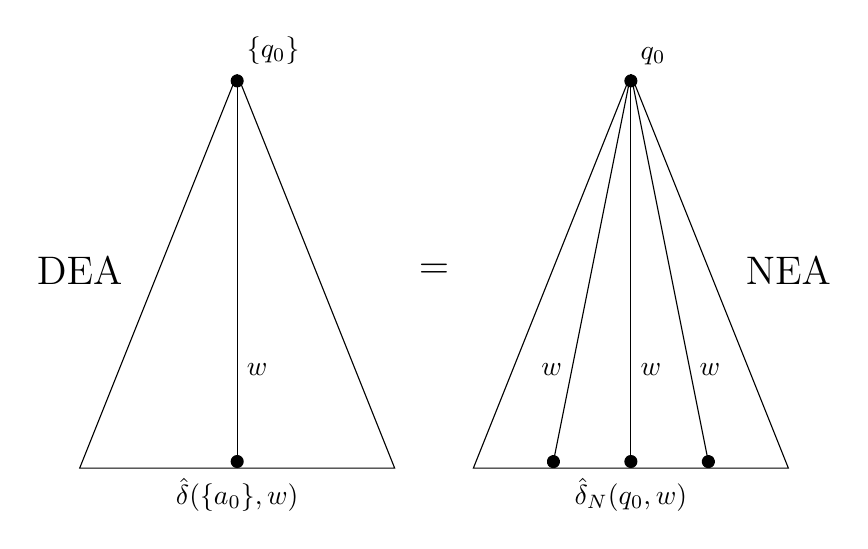
\begin{tikzpicture}
\draw (0,0) -- (2,-5) -- (-2,-5) -- (0,0);
\draw (5,0) -- (7,-5) -- (3,-5) -- (5,0);

\draw[*-*] (0,0) node[above right] {$\{q_0\}$} -- (0,-5) node[right, near end] {$w$} node[below] {$\hat{\delta} (\{a_0\}, w)$};

\draw[*-*] (5,0) node[above right] {$q_0$} -- (5,-5) node[right, near end] {$w$} node[below] {$\hat{\delta}_N (q_0, w)$};
\draw[-*] (5,0) -- (4,-5) node[left, near end] {$w$};
\draw[-*] (5,0) -- (6,-5) node[right, near end] {$w$};

\node at (-2,-2.5) {\Large{DEA}};
\node at (7,-2.5) {\Large{NEA}};
\node at (2.5,-2.5) {\Large{$=$}};
\end{tikzpicture}
\Img{GI-05.05.2009-IMG-3}

\subsection{GI(T)-05.05.2009-IMG-1}
\begin{tikzpicture}[->,>=stealth',shorten >=1pt,auto,node distance=2.8cm,semithick]
\node[state] at (187bp,305bp) (BD) {BD};
\node[state] at (158bp,136bp) (BE) {BE};
\node[state,accepting] at (52bp,117bp) (BF) {BF};
\node[state,accepting] at (106bp,361bp) (AE) {AE};
\node[state,accepting,initial,initial text=] at (80bp,244bp) (AD) {AD};
\node[state,accepting] at (203bp,418bp) (AF) {AF};
\node[state,accepting] at (143bp,28bp) (CF) {CF};
\node[state] at (233bp,199bp) (CE) {CE};
\node[state] at (246bp,86bp) (CD) {CD};

\tikzedge{AD}{BD}{1}{}{};
\tikzedge{AD}{AE}{0}{}{};

\tikzedge{BD}{AD}{1}{bend left}{};
\tikzedge{BD}{CE}{0}{}{};

\tikzedge{AE}{BD}{1}{}{};
\tikzedge{AE}{AF}{0}{}{};

\tikzedge{AF}{BD}{1}{}{};
\tikzloop{AF}{0}{above}{};

\tikzedge{CE}{CD}{1}{}{};
\tikzedge{CE}{BF}{0}{above}{};

\tikzedge{BF}{AD}{1}{}{};
\tikzedge{BF}{CF}{0}{bend left}{};

\tikzedge{CF}{CD}{1}{}{};
\tikzedge{CF}{BF}{0}{}{};

\tikzedge{BE}{AD}{1}{}{};
\tikzedge{BE}{CF}{0}{}{};

\tikzloop{CD}{1}{below}{};
\tikzedge{CD}{BE}{0}{}{};
\end{tikzpicture}
\Img{GI(T)-05.05.2009-IMG-1}
\section{06.05.2009}
\subsection{GI-06.05.2009-IMG-1}
\begin{tikzpicture}[->,>=stealth',shorten >=1pt,auto,node distance=2.8cm,semithick]
  \node[state,initial,initial text=] at (73bp,175bp) (A) {A};
  \node[state] at (152bp,203bp) (C) {C};
  \node[state] at (84bp,95bp) (B) {B};
  \node[state,accepting] at (57bp,23bp) (E) {E};
  \node[state] at (159bp,121bp) (D) {D};
  \node[state] at (154bp,283bp) (G) {G};
  \node[state,accepting] at (232bp,212bp) (F) {F};
  \node[state,accepting] at (231bp,116bp) (H) {H};
    
  \tikzedge{A}{B}{0}{}{};
  \tikzedge{A}{C}{1}{}{};
  
  \tikzedge{B}{E}{0}{}{};
  \tikzedge{B}{D}{1}{}{};
  
  \tikzedge{C}{F}{0}{}{};
  \tikzedge{C}{D}{1}{}{};
  
  \tikzedge{G}{C}{0,1}{}{};
  
  \tikzloop{D}{0,1}{below}{};
  \tikzloop{E}{0,1}{below}{};
  \tikzloop{F}{0,1}{above}{};
  \tikzloop{H}{0,1}{above}{};
\end{tikzpicture}
\Img{GI-06.05.2009-IMG-1}

\section{07.05.2009}
\subsection{GI(U)-07.05.2009-IMG-1}
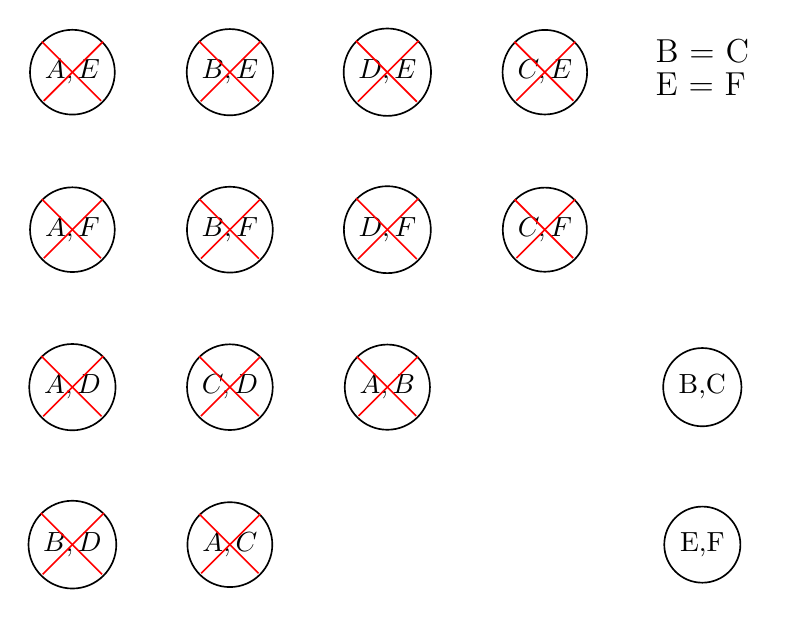
\begin{tikzpicture}[->,>=stealth',shorten >=1pt,auto,node distance=2.8cm,semithick]
\foreach \n/\pos/\np in {{A,E}/0/AE,{B,E}/1/BE,{D,E}/2/DE,{C,E}/3/CE}
{
\node[state] (\np) at (\pos*2,0) {$\n$};
\draw[color=red,-] (\np.north west) -- (\np.south east);
\draw[color=red,-] (\np.north east) -- (\np.south west);
}

\foreach \n/\pos/\np in {{A,F}/0/AF,{B,F}/1/BF,{D,F}/2/DF,{C,F}/3/CF}
{
\node[state] (\np) at(\pos*2,-2) {$\n$};
\draw[color=red,-] (\np.north west) -- (\np.south east);
\draw[color=red,-] (\np.north east) -- (\np.south west);
}

\foreach \n/\pos/\np in {{A,D}/0/AD,{C,D}/1/CD,{A,B}/2/AB}
{
\node[state] (\np) at(\pos*2,-4) {$\n$};
\draw[color=red,-] (\np.north west) -- (\np.south east);
\draw[color=red,-] (\np.north east) -- (\np.south west);
}

\foreach \n/\pos/\np in {{B,D}/0/BD,{A,C}/1/AC}
{
\node[state] (\np) at(\pos*2,-6) {$\n$};
\draw[color=red,-] (\np.north west) -- (\np.south east);
\draw[color=red,-] (\np.north east) -- (\np.south west);
}

\node[state] (BC) at(8,-4) {B,C};
\node[state] (EF) at(8,-6) {E,F};

\tikzedge{AC}{BF}{0}{bend left}{left, near start};
\tikzedge{AD}{CD}{1}{}{above};
\tikzedge{AD}{BD}{1}{}{right};
\tikzedge{AB}{CD}{1}{}{below};
\tikzedge{CD}{DF}{1}{}{left};
\tikzedge{AB}{BE}{0}{}{above, near end};
\tikzedge{BD}{DE}{0}{bend left}{right, near end};
\tikzedge{BC}{EF}{0}{}{right};
\tikzloop{EF}{1,0}{below}{right};

\node at (8,0) {
\begin{tabular}{l}
\large{B = C}\\
\large{E = F}
\end{tabular}};
\end{tikzpicture}
\Img{GI(U)-07.05.2009-IMG-1}

\subsection{GI(U)-07.05.2009-IMG-2}
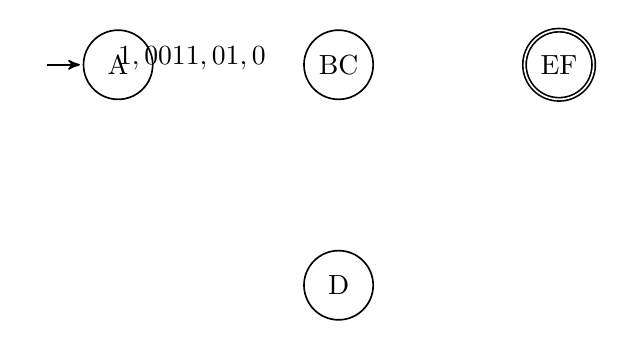
\begin{tikzpicture}[->,>=stealth',shorten >=1pt,auto,node distance=2.8cm,semithick]
\node[state,initial,initial text=] (A) {A};
\node[state] (BC) [right of=A] {BC};
\node[state,accepting] (EF) [right of=BC] {EF};
\node[state] (D) [below of=BC] {D};

\tikzedge{A}{BC}{$1, 0$}{}{above};
\tikzedge{BC}{EF}{$0$}{}{above};
\tikzedge{BC}{D}{$1$}{}{right};
\tikzloop{D}{$1, 0$}{below}{right};
\tikzloop{EF}{$1, 0$}{above}{right};
\end{tikzpicture}
\Img{GI(U)-07.05.2009-IMG-2}

\subsection{GI(U)-07.05.2009-IMG-3}
\begin{table}[h]
\centering
\begin{tabular}{c|c|c|c|}
&&0&1\\\hline
\RM{1}&A&\RM{1}&\RM{1}\\
&A&\RM{2}&\RM{1}\\
&B&\RM{2}&\RM{1}\\
&C&\RM{2}&\RM{1}\\
&D&\RM{1}&\RM{1}\\\hline
\RM{2}&E&\RM{2}&\RM{2}\\
&F&\RM{2}&\RM{2}
\end{tabular}
$\Rightarrow$
\begin{tabular}{c|c|c|c|}
&&0&1\\\hline
\RM{1}&A&\RM{2}&\RM{2}\\
&D&\RM{1}&\RM{1}\\\hline
\RM{2}&B&\RM{3}&\RM{1}\\
&C&\RM{3}&\RM{1}\\\hline
\RM{3}&E&\RM{3}&\RM{3}\\
&F&\RM{3}&\RM{3}
\end{tabular}
$\Rightarrow$
\begin{tabular}{c|c|c|c|}
&&0&1\\\hline
\RM{1}&A&\RM{3}&\RM{3}\\\hline
\RM{2}&D&\RM{2}&\RM{2}\\\hline
\RM{3}&B&\RM{4}&\RM{2}\\
&C&\RM{4}&\RM{2}\\\hline
\RM{4}&E&\RM{4}&\RM{4}\\
&F&\RM{4}&\RM{4}\\
\end{tabular}
\end{table}
\Img{GI(U)-07.05.2009-TAB-3}

\subsection{GI(U)-07.05.2009-IMG-4}
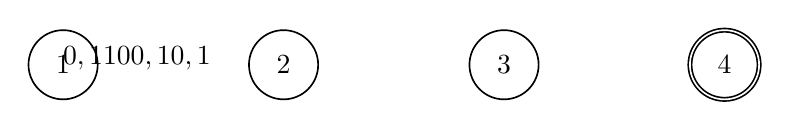
\begin{tikzpicture}[->,>=stealth',shorten >=1pt,auto,node distance=2.8cm,semithick]
\node[state] (1) {\RM{1}};
\node[state] (2) [right of=1] {\RM{2}};
\node[state] (3) [right of=2] {\RM{3}};
\node[state,accepting] (4) [right of=3] {\RM{4}};

\tikzedge{1}{3}{$0, 1$}{bend left}{above};
\tikzedge{3}{2}{$1$}{}{above};
\tikzedge{3}{4}{$0$}{}{above};
\tikzloop{2}{$0, 1$}{below}{right};
\tikzloop{4}{$0, 1$}{above}{right};
\end{tikzpicture}
\Img{GI(U)-07.05.2009-IMG-4}

\section{12.05.2009}
\subsection{GI-12.05.2009-IMG-1}
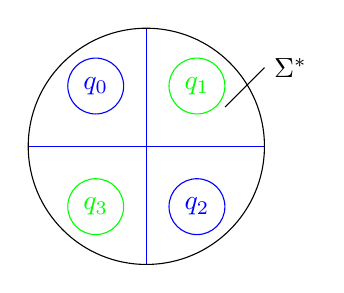
\begin{tikzpicture}
\draw[color=blue] (0,1.5) -- (0,-1.5);
\draw[color=blue] (0,0) -- (-180:1.5);
\draw[color=blue] (0,0) -- (0:1.5);
\draw (0,0) circle (1.5);
\draw (1,0.5) -- (1.5,1) node[right] {$\Sigma^*$};
\node[shape=circle,color=blue,draw] at (130:1) {$q_0$};
\node[shape=circle,color=green,draw] at (50:1) {$q_1$};
\node[shape=circle,color=blue,draw] at (-50:1) {$q_2$};
\node[shape=circle,color=green,draw] at (-130:1) {$q_3$};
\end{tikzpicture}
\Img{GI-12.05.2009-IMG-1}

\subsection{GI-12.05.2009-IMG-2}
\begin{tikzpicture}[->,>=stealth',shorten >=1pt,auto,node distance=2.8cm,semithick]
\node[state,initial,initial text=,accepting] (A) {$\epsilon$};
\node[state] (B) [right of=A] {};
\node[state] (C) [right of=B] {};
\node[state] (D) [below of=C] {};
\node[state] (F) [below of=D] {};
\node[state] (E) [left of=F] {};
\node[state] (DS) [left of=E] {DS};
\node (dots) [right of=C] {\dots};

\tikzedge{A}{B}{0}{}{};
\tikzedge{A}{DS}{1}{}{};

\tikzedge{B}{C}{0}{}{};
\tikzedge{B}{E}{1}{}{};

\tikzedge{C}{D}{1}{}{};

\tikzedge{D}{DS}{0}{}{};
\tikzedge{D}{F}{1}{}{};

\tikzedge{E}{DS}{0,1}{}{};

\tikzedge{F}{DS}{0,1}{bend left}{};

\tikzloop{DS}{0,1}{left}{};

\end{tikzpicture}
\Img{GI-12.05.2009-IMG-2}

\subsection{GI-12.05.2009-IMG-3}
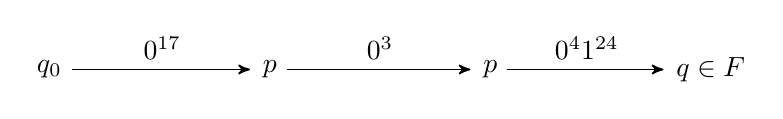
\begin{tikzpicture}[->,>=stealth',shorten >=1pt,auto,node distance=2.8cm,semithick]
\node (q0) {$q_0$};
\node (p1) [right of=q0] {$p$};
\node (p2) [right of=p1] {$p$};
\node (q1) [right of=p2] {$q \in F$};

\path[->] (q0) edge node {$0^{17}$} (p1);
\path[->] (p1) edge node {$0^{3}$} (p2);
\path[->] (p2) edge node {$0^{4} 1^{24}$} (q1);
\end{tikzpicture}
\Img{GI-12.05.2009-IMG-3.1}

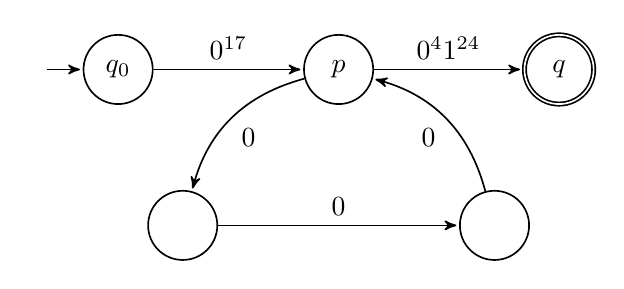
\begin{tikzpicture}[->,>=stealth',shorten >=1pt,auto,node distance=2.8cm,semithick]
\node[state,initial,initial text=] (q0) {$q_0$};
\node[state] (p) [right of=q0] {$p$};
\node[state,accepting] (q) [right of=p] {$q$};
\node[state] (p1) [below left of=p]{};
\node[state] (p2) [below right of=p]{};

\path[->] (q0) edge node {$0^{17}$} (p);
\path[->] (p) edge node {$0^{4} 1^{24}$} (q);
\path[->] (p) edge [bend right] node {$0$} (p1);
\path[->] (p1) edge node {$0$} (p2);
\path[->] (p2) edge [bend right] node {$0$} (p);
\end{tikzpicture}
\Img{GI-12.05.2009-IMG-3.2}

\subsection{GI-12.05.2009-IMG-4}
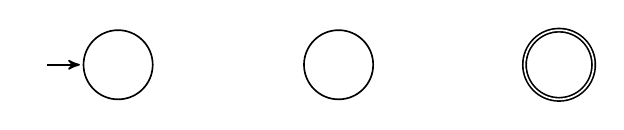
\begin{tikzpicture}[->,>=stealth',shorten >=1pt,auto,node distance=2.8cm,semithick]
\node[state,initial,initial text=] (initial) {};
\node[state] (n1) [right of=initial] {};
\node[state,accepting] [right of=n1] (n2) {};

\tikzedge{initial}{n1}{0}{}{};
\tikzedge{n1}{n2}{w}{}{};
\tikzloop{n1}{v}{above}{};
\end{tikzpicture}
\Img{GI-12.05.2009-IMG-4}

\section{26.05.2009}
\subsection{GI-26.05.2009-IMG-1}
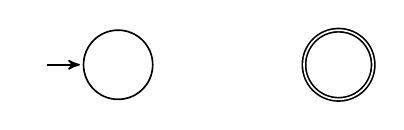
\begin{tikzpicture}[->,>=stealth',shorten >=1pt,auto,node distance=2.8cm,semithick]
\node[state,initial,initial text=] (s) {};
\node[state, accepting] (a) [right of=s] {};
\tikzedge{s}{a}{a}{}{};
\end{tikzpicture}
\Img{GI-26.05.2009-IMG-1}

\subsection{GI-26.05.2009-IMG-2}
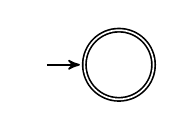
\begin{tikzpicture}[->,>=stealth',shorten >=1pt,auto,node distance=2.8cm,semithick]
\node[state, accepting,initial,initial text=] {};
\end{tikzpicture}
\Img{GI-26.05.2009-IMG-2}

\subsection{GI-26.05.2009-IMG-3}
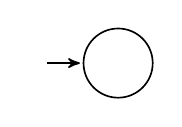
\begin{tikzpicture}[->,>=stealth',shorten >=1pt,auto,node distance=2.8cm,semithick]
\node[state,initial,initial text=] {};
\end{tikzpicture}
\Img{GI-26.05.2009-IMG-3}

\subsection{GI-26.05.2009-IMG-4}
\begin{tikzpicture}[->,>=stealth',shorten >=1pt,auto,node distance=2cm,semithick]
\draw (0,-2) rectangle (2,2);
\draw (4,-2) rectangle (6,2);

\node[state,initial,initial text=,fill=white] at (0,0) (m1s) {};
\node[state,fill=white] (m1n1) at (2,1.5) {};
\node[state,fill=white] (m1n2) at (2,-1.5) {};

\node[state,fill=white] (m2s) at (4,0) {};
\node[state,accepting,fill=white] (m2n1) at (6,1.5) {};
\node[state,accepting,fill=white] (m2n2) at (6,-1.5) {};

\tikzedge{m1n1}{m2s}{\epsilon}{}{};
\tikzedge{m1n2}{m2s}{\epsilon}{}{};

\node[node distance=1cm, right of=m1s] {\Large{$M_1$}};
\node[node distance=1cm, right of=m2s] {\Large{$M_2$}};

\end{tikzpicture}
\Img{GI-26.05.2009-IMG-4}

\subsection{GI-26.05.2009-IMG-5}
\begin{tikzpicture}[->,>=stealth',shorten >=1pt,auto,node distance=2.8cm,semithick]

\end{tikzpicture}
\Img{GI-26.05.2009-IMG-5}

\subsection{GI-26.05.2009-IMG-6}
\begin{tikzpicture}[->,>=stealth',shorten >=1pt,auto,node distance=2cm,semithick]
\draw (0,-2) rectangle (2,2);

\node[state,fill=white] at (0,0) (m1s) {};
\node[state,fill=white] (m1n1) at (2,1.5) {};
\node[state,fill=white] (m1n2) at (2,0) {};
\node[state,fill=white] (m1n3) at (2,-1.5) {};
\node[state,initial,initial text=] (start) [left of=m1s] {};
\node[state,accepting] (end) [right of=m1n2] {};

\tikzedge{m1n1}{end}{\epsilon}{}{};
\tikzedge{m1n2}{end}{\epsilon}{}{};
\tikzedge{m1n3}{end}{\epsilon}{}{};
\tikzedge{start}{end}{\epsilon}{bend left}{};
\tikzedge{end}{start}{\epsilon}{bend left}{};
\tikzedge{start}{m1s}{\epsilon}{}{};

\node[node distance=1cm, right of=m1s] {\Large{$M_1$}};

\end{tikzpicture}
\Img{GI-26.05.2009-IMG-6}

\subsection{GI-26.05.2009-IMG-7}
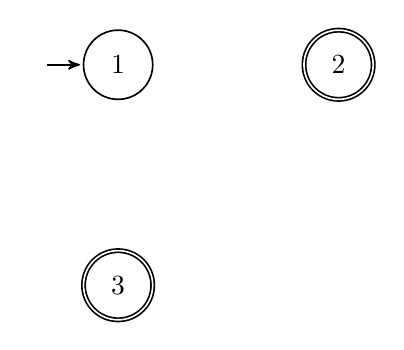
\begin{tikzpicture}[->,>=stealth',shorten >=1pt,auto,node distance=2.8cm,semithick]
\node[state, initial, initial text=] (1) {1};
\node[state, accepting] (2) [right of=1] {2};
\node[state, accepting] (3) [below of=1] {3};

\tikzloop{2}{1}{above}{};
\tikzedge{1}{2}{0}{bend left}{};
\tikzedge{2}{1}{0}{bend left}{};

\tikzedge{1}{3}{1}{bend left}{};
\tikzedge{3}{1}{1}{bend left}{};

\tikzedge{3}{2}{0}{}{};
\end{tikzpicture}
\Img{GI-26.05.2009-IMG-7}

\subsection{GI-26.05.2009-IMG-8}
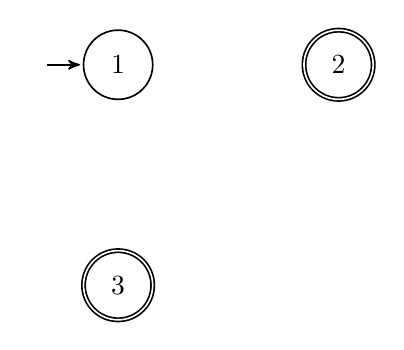
\begin{tikzpicture}[->,>=stealth',shorten >=1pt,auto,node distance=2.8cm,semithick]
\node[state, initial, initial text=] (1) {1};
\node[state, accepting] (2) [right of=1] {2};
\node[state, accepting] (3) [below of=1] {3};

\tikzloop{2}{1}{above}{};
\tikzedge{1}{2}{0}{bend left}{};
\tikzedge{2}{1}{0}{bend left}{};

\tikzedge{1}{3}{1}{bend left}{};
\tikzedge{3}{1}{1}{bend left}{};

\tikzedge{3}{2}{0}{}{};
\end{tikzpicture}
\Img{GI-26.05.2009-IMG-8}

\subsection{GI-26.05.2009-IMG-9}
\begin{tikzpicture}[->,>=stealth',shorten >=1pt,auto,node distance=2.8cm,semithick]
\node[state,color=blue] (qi) {$q_i$};
\node[state,color=red] (qrip) [above right of=qi] {$q_{rip}$};
\node[state,color=green] (qj) [below right of=qrip] {$q_j$};

\tikzedge{qi}{qrip}{r_1}{}{};
\tikzedge{qi}{qj}{r_4}{}{};
\tikzedge{qrip}{qj}{r_3}{}{};
\tikzloop{qrip}{r_2}{below}{};

\node[state,color=blue] (qi2) [below of=qi, node distance=1.5cm] {$q_i$};
\node[state,color=green] (qj2) [below of=qj, node distance=1.5cm] {$q_j$};

\tikzedge{qi2}{qj2}{r_4 + r_1 \cdot (r_2)^* \cdot r_2}{}{};
\end{tikzpicture}
\Img{GI-26.05.2009-IMG-9}

\subsection{GI-26.05.2009-IMG-11}
\begin{tikzpicture}[->,>=stealth',shorten >=1pt,auto,node distance=2.8cm,semithick]
\node[state,initial,initial text=] (qs) {$q_s$};
\node[state] (2) [above right of=qs] {$2$};
\node[state] (3) [below right of=qs] {$3$};
\node[state] (qa) [above right of=3] {$q_a$};

\tikzloop{3}{11 \textcolor{gray}{+ (10 + 0)(1 + 00)^* \cdot (01)}}{below}{};
\tikzloop{2}{1 + 00}{above}{};

\tikzedge{qs}{2}{0}{}{};
\tikzedge{qs}{3}{1 \textcolor{gray}{+ 0 (1 + 00)^* 01} = r_1}{}{};
\path[->,color=gray] (qs) edge[bend right] node {$0 \cdot (1 + 00)^* \cdot \epsilon \textcolor{black}{= r_4}$} (qa);

\tikzedge{2}{qa}{\epsilon}{}{};
\tikzedge{2}{3}{01}{bend right}{};

\tikzedge{3}{2}{10 + 0}{bend right}{};
\tikzedge{3}{qa}{\epsilon \textcolor{gray}{+(10 + 0) (1 + 00)} = r_2}{}{};
\end{tikzpicture}
\Img{GI-26.05.2009-IMG-11}

\chapter{Mathematik 2}
\section{22.04.2009}
\subsection{MA2-22.04.2009-IMG-2}
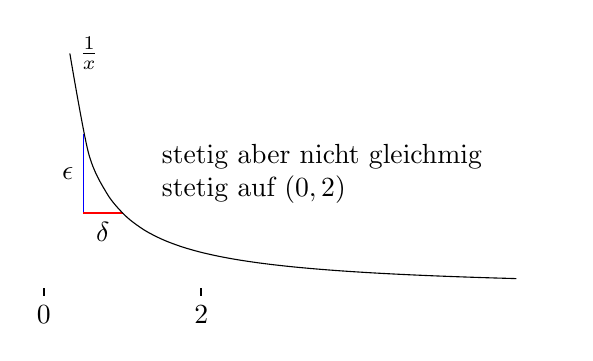
\begin{tikzpicture}[domain=6:0.33]
\tikzcoor[x][]{6}{3}
\foreach \x in {0,2}
	\draw[thick] (\x,-0.05) node[below] {$\x$} -- (\x,0.05); 

\draw[color=blue] (0.5,{1/0.5}) -- (0.5, {1/0.5 - 1}) node[left, midway, color=black] {$\epsilon$};
\draw[color=red] (0.5,{1/0.5 - 1}) -- (1, {1/0.5 - 1}) node[below, midway, color=black] {$\delta$};
\draw plot[smooth] (\x,{1/\x}) node[right] {$\frac{1}{x}$};
\node[text width=5cm] at (4,1.5) {stetig aber nicht gleichmig stetig auf $(0,2)$};
\end{tikzpicture}
\Img{MA2-22.04.2009-IMG-2}

\subsection{MA2-22.04.2009-IMG-3}
\begin{tikzpicture}[scale=2.0]
\tikzcoor[x][]{3}{1.5}
\foreach \x in {0,1}
	\node[left] at (0,\x) {$\x$}; 

\draw[thick,(-,color=blue] (0,1) -- (2,1);
\draw[thick,[-,color=blue] (0,0) -- (-1,0);
\end{tikzpicture}
\Img{MA2-22.04.2009-IMG-3}

\subsection{MA2-22.04.2009-IMG-4}
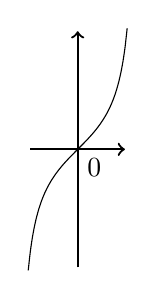
\begin{tikzpicture}[scale=0.5]
\draw[thick,->] (0,-3) -- (0,3);
\draw[thick,->] (-1.2,0) -- (1.2,0);
\draw plot[smooth,domain=0:pi/2.5] (\x,{tan(\x r)});
\draw plot[smooth,domain=0:-pi/2.5] (\x,{-tan(-\x r)});
\node at (0,0) [below right] {$0$};
\end{tikzpicture}
\Img{MA2-22.04.2009-IMG-4}

\section{23.04.2009}
\subsection{MA2-23.04.2009-IMG-1}
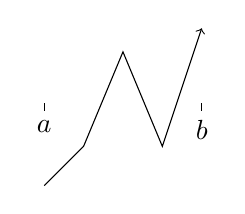
\begin{tikzpicture}
\tikzcoor[x][]{3.5}{1.5}

\foreach \x/\y in{1/a,3/b}
	\draw (\x,-0.05) node[below] {$\y$} -- (\x,0.05);

\draw[->] (1,-1) -- (1.5,-0.5) -- (2, 0.7) -- (2.5,-0.5) -- (3,1);
\end{tikzpicture}
\Img{MA2-23.04.2009-IMG-1}

\subsection{MA2-23.04.2009-IMG-2}
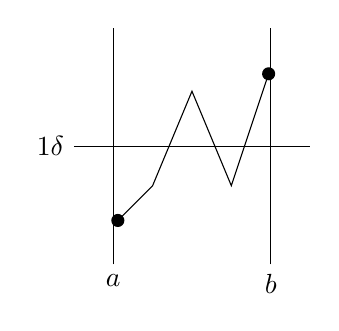
\begin{tikzpicture}

\draw (0.5,0) node[left] {$1 \delta$} -- (3.5,0);
\draw[*-*] (1,-1) -- (1.5,-0.5) -- (2, 0.7) -- (2.5,-0.5) -- (3,1);
\draw (1,-1.5) node[below] {$a$} -- (1,1.5);
\draw (3,-1.5) node[below] {$b$} -- (3,1.5);
\end{tikzpicture}
\Img{MA2-23.04.2009-IMG-2}

\subsection{MA2-23.04.2009-IMG-3}
\begin{tikzpicture}
\tikzcoor[][]{2}{2}

\foreach \x in{0,1}
	\draw[thick] (\x,-0.05) node[below] {$\x$} -- (\x,0.05);

\draw plot[smooth, domain=0.15:2] (\x,{1/\x * 0.3});

\end{tikzpicture}
\Img{MA2-23.04.2009-IMG-3}

\subsection{MA2-23.04.2009-IMG-4}
\begin{tikzpicture}[scale=0.5]
\tikzcoor[][]{12.566}{1.5}
\draw[thick] (0,-1.5) -- (0,1.5);

\draw[thick] (6.283,-0.05) node[below] {$\frac{\pi}{2}$} -- (6.283,0.05);

\draw plot[smooth, domain=0:12.566] (\x,{sin(\x r)});

\end{tikzpicture}
\Img{MA2-23.04.2009-IMG-4}

\subsection{MA2-23.04.2009-IMG-5}
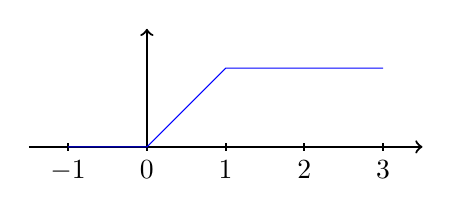
\begin{tikzpicture}
\draw[thick, ->] (-1.5,0) -- (3.5,0);
\draw[thick, ->] (0,0) -- (0,1.5);

\foreach \x in {-1,0,...,3}
	\draw[thick] (\x,-0.05) node[below] {$\x$} -- (\x,0.05);

\draw[blue] (-1,0) -- (0,0) -- (1,1) -- (2,1) -- (3,1);
\end{tikzpicture}
\Img{MA2-23.04.2009-IMG-5}

\section{28.04.2009}
\subsection{MA2-28.04.2009-IMG-1}
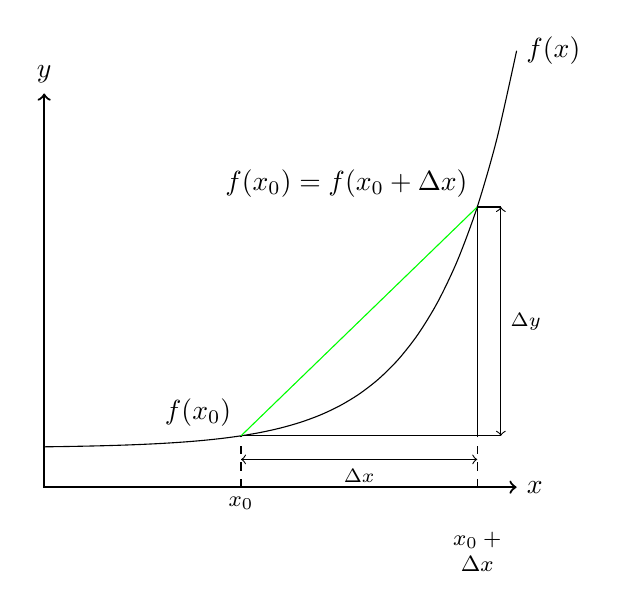
\begin{tikzpicture}[domain=0:6]
\draw[<->,thick] (0,5) node[above] {$y$} -- (0,0) -- (6,0) node[right] {$x$};
\draw plot[smooth] (\x,{exp(\x)/80 + 0.5}) node[right] {$f(x)$};
\draw (2.5,{exp(2.5)/80 + 0.5}) -- (5.5,{exp(2.5)/80 + 0.5}) -- (5.5,{exp(5.5)/80 + 0.5});
\draw[color=green] (2.5,{exp(2.5)/80 + 0.5}) node[above left, color=black] {$f(x_0)$} -- (5.5,{exp(5.5)/80 + 0.5}) node[above left, color=black] {$f(x_0) = f(x_0 + \Delta x)$};
\draw[dashed] (2.5,0) node[below] {\footnotesize{$x_0$}} -- (2.5,{exp(2.5)/80 + 0.5});
\draw[dashed] (5.5,0) node[below, text width=7mm] {\begin{center}\footnotesize{$x_0 + \Delta x$}\end{center}} -- (5.5,{exp(5.5)/80 + 0.5});

\draw[<->] (2.5,{exp(2.5)/80 + 0.2}) -- (5.5,{exp(2.5)/80 + 0.2}) node[below, midway] {\scriptsize{$\Delta x$}};
\draw (5.5,{exp(2.5)/80 + 0.5}) -- (5.8,{exp(2.5)/80 + 0.5});
\draw (5.5,{exp(5.5)/80 + 0.5}) -- (5.8,{exp(5.5)/80 + 0.5});
\draw[<->] (5.8,{exp(2.5)/80 + 0.5}) -- (5.8,{exp(5.5)/80 + 0.5}) node[right, midway] {\scriptsize{$\Delta y$}};
\end{tikzpicture}
\Img{MA2-28.04.2009-IMG-1}

\section{07.05.2009}
\subsection{MA2-07.05.2009-IMG-1}
\begin{tikzpicture}[decoration=brace]
\tikzcoor{9}{6}
\draw[thick] (1.5,-0.05) node[below] {$a$} -- (1.5,0.05);
\draw[thick] (7,-0.05) node[below] {$b$} -- (7,0.05);
\draw[thick] (5.5,-0.05) node[below] {$\xi$} -- (5.5,0.05);
\draw[thick] (-0.05,1) node[left] {$f(a)$} -- (0.05,1);
\draw[thick] (-0.05,4.5) node[left] {$f(b)$} -- (0.05,4.5);

\draw[dashed] (1.5,0) -- (1.5,1);
\draw[dashed] (7,0) -- (7,4.5);
\draw[dashed] (0,1) -- (7,1);
\draw[dashed] (0,4.5) -- (7,4.5);
\draw[blue] (1.5,1) -- (7,4.5);

\draw[out=0, in=190] (1.5,1) to (4.75,1.3) [out=10, in=240] to (7,4.5) node[above] {$f(b)$};

\draw[decorate] (7.2,4.5) -- (7.2,1) node[right, midway] {$f(b) - f(a)$};
\end{tikzpicture}
\Img{MA2-07.05.2009-IMG-1}


\end{document}
